\documentclass[a4paper,11pt,fleqn]{article}%fleqn pour aligner les equations à gauche
\usepackage{../../Styles/Cours}


\newcommand{\chnum}{Chapitre 12}
\newcommand{\chtitle}{Pression d'un gaz}
\newcommand{\dtype}{AE1}

\begin{document}
	\maketitle
Contrairement aux liquides, les gaz sont compressibles, c’est à dire que, dans un récipient fermé et rempli de gaz, on peut changer son volume et cela entraînera une variation de pression. On peut ainsi questionner le lien entre pression et volume pour un gaz.
\begin{figure}[h!]
	\begin{minipage}{.48\linewidth}
		Dans le montage expérimental suivant, on dispose d’une seringue graduée reliée par un tube flexible à un pressiomètre qui mesure la pression de l’air emprisonné dans la seringue.
	\end{minipage}\hspace{2em}
	\begin{minipage}{.48\linewidth}
		\centering 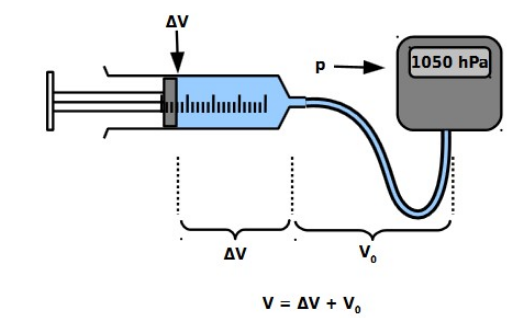
\includegraphics[width = .7\linewidth]{Ressources/1SPE_C12_AE1_Fig1.png}
	\end{minipage}
\end{figure}

La pression se mesure en pascal (\unit{\pascal}) mais on la mesure presque toujours en hectopascal (\unit{\hecto\pascal}). Avec \SI{1}{\hecto\pascal} = \SI{100}{\pascal}.Le manomètre affiche la pression à l’intérieur de la seringue qui est égale, au début de l’expérience, à la pression atmosphérique notée $P_0$.
\begin{itemize}
	\item Le piston est normalement placé sur un volume de 30 mL. Relever la pression correspondante et la noter dans le tableau ci-dessous.
	\item Pousser ou tirer le piston sur les volumes indiqués dans le tableau suivant. Relever les pressions correspondantes et les noter dans le tableau.
\end{itemize}
\begin{center}
	\begin{tabular}{|>{\centering}m{.15\linewidth}|>{\centering}m{.08\linewidth}|>{\centering}m{.08\linewidth}|>{\centering}m{.08\linewidth}|>{\centering}m{.08\linewidth}|>{\centering}m{.08\linewidth}|>{\centering}m{.08\linewidth}|>{\centering}m{.08\linewidth}|>{\centering\arraybackslash}m{.08\linewidth}|}
		\hline
		Volume (\unit{\milli\liter}) & \num{15} & \num{20} & \num{25} & \num{30} & \num{35} & \num{40} & \num{45} & \num{50}\\
		\hline
		Pression (\unit{\hecto\pascal}) & & & & & & & & \\
		\hline
	\end{tabular}
\end{center}

\begin{enumerate}
	\item Recopier les valeurs mesurées en convertissant le volume en \unit{\meter\cubed} et la pression en \unit{\pascal}.
\end{enumerate}

\begin{center}
	\begin{tabular}{|>{\centering}m{.15\linewidth}|>{\centering}m{.08\linewidth}|>{\centering}m{.08\linewidth}|>{\centering}m{.08\linewidth}|>{\centering}m{.08\linewidth}|>{\centering}m{.08\linewidth}|>{\centering}m{.08\linewidth}|>{\centering}m{.08\linewidth}|>{\centering\arraybackslash}m{.08\linewidth}|}
		\hline
		Volume (\unit{\cubic\meter}) & & & & & & & & \\
		\hline
		Pression (\unit{\pascal}) & & & & & & & & \\
		\hline
	\end{tabular}
\end{center}

\begin{itemize}
	\item Dans un tableur (ordinateur ou calculatrice) recopier le tableau précédent
	\item Tracer la courbe représentant $P$ en fonction de $V$.
\end{itemize}

\begin{enumerate}[resume]
	\item La pression d'un gaz est elle proportionnelle au volume occupé par celui-ci ? Justifier.
\end{enumerate}

En physique on cherche toujours à obtenir une droite à partir ces mesures car on peut en déduire une équation qui deviendra une formule reliant deux grandeurs. Puisque les fonctions mathématiques les plus courantes sont les fonctions du second degré ($ax^2 +bx +c$), la fonction inverse ($\dfrac{1}{x}$) et la fonction exponentielle ($e^x$), insérer trois colonnes supplémentaires correspondant aux valeurs de $V^2$, $\dfrac{1}{V}$ et $e^V$. 

\begin{itemize}
	\item Tracer successivement ces trois fonctions.
\end{itemize}

\begin{enumerate}[resume]
	\item Laquelle des fonctions représentées donne une droite ?
	\item Déterminer l'équation de la droite obtenue.
\end{enumerate}

Le résultat obtenu se met sous la forme $P\cdot V =cste$,  c'est la loi de Mariotte.
\begin{enumerate}[resume]
	\item Calculer cette constante dans notre cas.
\end{enumerate}
\end{document}